% ****** Start of file apssamp.tex ******
%
%   This file is part of the APS files in the REVTeX 4.2 distribution.
%   Version 4.2a of REVTeX, December 2014
%
%   Copyright (c) 2014 The American Physical Society.
%
%   See the REVTeX 4 README file for restrictions and more information.
%
% TeX'ing this file requires that you have AMS-LaTeX 2.0 installed
% as well as the rest of the prerequisites for REVTeX 4.2
%
% See the REVTeX 4 README file
% It also requires running BibTeX. The commands are as follows:
%
%  1)  latex bifurcations.tex
%  2)  bibtex bifurcations
%  3)  latex bifurcations.tex
%  4)  latex bifurcations.tex
%
\documentclass[%
 % reprint,
10pt,
superscriptaddress,
twocolumn,
%groupedaddress,
%unsortedaddress,
%runinaddress,
%frontmatterverbose,
%preprint,
%preprintnumbers,
%nofootinbib,
%nobibnotes,
%bibnotes,
 amsmath,amssymb,
 aps,prx,
%pra,
%prb,
%rmp,
%prstab,
%prstper,
%floatfix,
]{revtex4-2}

\usepackage{graphicx}% Include figure files
\usepackage{dcolumn}% Align table columns on decimal point
% \usepackage{bm}% bold math
\usepackage{xcolor}
\usepackage{hyperref}% add hypertext capabilities
\usepackage{siunitx}% SI units
\usepackage{physics}
\usepackage[utf8]{inputenc}
\usepackage[T1]{fontenc}
\usepackage{lmodern}
\usepackage{amsmath,amsfonts,amssymb}
\usepackage{natbib}


\AtBeginDocument{\renewcommand*{\d}{\mathop{\kern0pt\mathrm{d}}\!{}}}
\graphicspath{{Figures/}} % set default figure path to figures/, if we store figure files in figures/, we only need to put file name in \includegraphics{filename.pdf}. For supported formats, e.g. pdf and jpg, we can omit the extensions. This enhances the readability of the source.

% Some formatting guidelines
% 1. Start a new line (\n) for each sentence. This is good for synctex (click pdf and find the line in tex), and also good for Git when comparing versions.
% 2. Communicate thoughts in comments. For example, if you think a figure of something is needed but missing some where, put a comment and describe the needs.
% 3. Colored text: I use red text to emphasize that the claim is not fully backed by our results. The wording may be modified in the future.
% 4. Figure crossref: at the beginning of a sentence, use "Figure~\ref{}". Otherwise, use "Fig.~\ref{}". Note that the "~" is to prevent line breaking in the middle of the crossref.

\begin{document}

\preprint{APS/123-QED}

\title{Active Nematics at Bifurcations}% Force line breaks with \\

\author{Zhengyang Liu}
\author{Claire Doré}
\affiliation{Laboratoire Gulliver, UMR 7083 CNRS, ESPCI Paris, PSL Research University, 75005 Paris, France.}

\author{Antonio Tavera-Vazquez}
\affiliation{Laboratoire Gulliver, UMR 7083 CNRS, ESPCI Paris, PSL Research University, 75005 Paris, France.}
\affiliation{Pritzker School of Molecular Engineering, University of Chicago, Chicago, IL 60637, USA.}

\author{Teresa Lopez-Leon}
\affiliation{Laboratoire Gulliver, UMR 7083 CNRS, ESPCI Paris, PSL Research University, 75005 Paris, France.}
\date{\today}


\begin{abstract}

Under lateral confinement, active matter self-organize into coherent flows. 
Such behavior implies the possibility of achieving logical operations in properly designed channel networks. 
Bifurcations are a key ingredient in channel networks.
Understanding active matter behavior at bifurcations is therefore an important step towards a proper channel network design.
In this paper, we experimentally explore active matter behavior at bifurcations using the microtubule-kinesin model system. 
Specifically, we compare the effects of channel length, ratchets and turning angles. 
Our results suggest that ratchets and turning angles help establish unambiguous polarized flow states.
In contrast, channel length is a less relevant factor, which results in more frequently changing flow states.
Our experiment is the first step to understanding active nematic flows in complex channel networks.
The result lays the foundation for active matter logic and computation.

\end{abstract}

\keywords{active matter logic, confinement, active nematics, ratchet, bifurcation}

\maketitle

\section{Introduction}

Active matter flows spontaneously under channel confinement, forming coherent flows  \cite{Wioland2016,Wu2017,Morin2018,Hardouin2019,Hardouin2020}. 
Such behavior implies several possibile applications of active matter, including serving as micro-scale transport, soft robotics and active matter logic \cite{Thampi2022,Woodhouse2017}.
Boundary-mediated control has been shown effective in manipulating active matter in both experiments \cite{Lushi2014,Wioland2016,Wioland2016,Wu2017,Morin2018,Liu2019,Ross2019,Hardouin2019} and simulations \cite{Voituriez2005,Marenduzzo2007,Shendruk2017,Vaidya2024}.
As of now, most studies have focused on the behavior of active matter in stand-alone smooth channels, which showed that active flows were intrinsically bistable \cite{Wu2017,Morin2018}.
However, to realize the full potential of active matter channel flows, it is necessary to study the behavior of active matter in channel networks and with asymmertic geometries, as suggested in the pioneering active matter logic work by \citet{Woodhouse2017}.
Very recently, channel networks attract more attention, and frustrated flow states have been investigated in coupled annular rings \cite{Hardouin2020} and large honeycomb-like networks \cite{Jorge2024}.
The other essential component of active matter logic is the diode channel, which only permits flow in one direction.
While a few early works have hinted or employed asymmetric geometries, such as a kink or an array of ratchet teeth, to steer active matter flows \cite{ElizabethHulme2008,DiLeonardo2010,Wu2017,Hardouin2020,Ray2023,Vaidya2024}, a systematic study of asymmetric channels in the context of channel networks is still missing. 

% Spontaneous flow under channel confinement is a phenomenon observed in various active matter systems \cite{Lushi2014,Wioland2016,Wu2017,Duclos2017,Morin2018,Hardouin2020}.
% Due to its ubiquitous and robustness, active matter holds significant potential for many applications, especially in the fields of microfluidics and soft robotics \cite{Hardouin2020}.
% Among the various proposed applications, active flow networks (AFN) are particularly interesting \cite{Woodhouse2016,Woodhouse2017}.
% AFNs are networks of channels where active matter flows.
% The most notable feature of AFNs is the potential capability of achieving logical operations, such as AND and OR, which enables the combination of mass transport and intelligence in a single circuit system. 
% \citet{Woodhouse2017} proposed to use a Landau-type bistable potential to model the phenomenon. 
% Combining mass conservation and diode channel which only permits flow in certain direction, they derived a theoretical framework of AFNs that can achieve logical operations.

% \begin{figure}[!h]
%     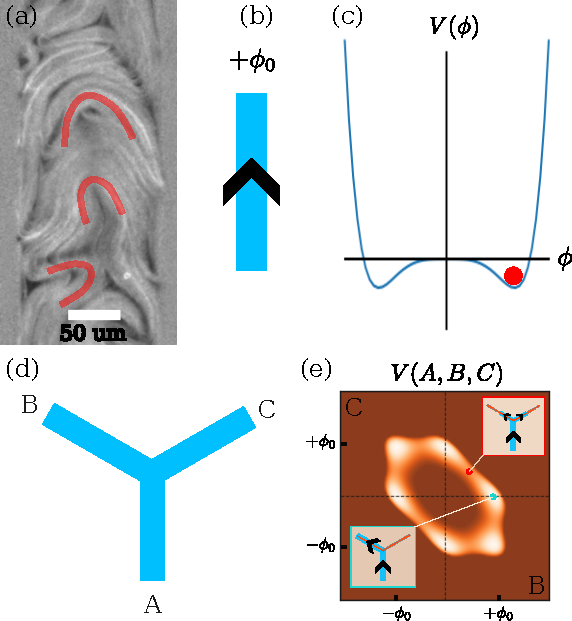
\includegraphics[width=0.45\textwidth]{1-bifurcation-question}
%     \caption{
%     \textbf{What do active nematics do in straight channels and bifurcations?}
%     (a) Spontaneous directed flow in a straight channel.
%     (b) A schematic diagram of the directed flow in a straight channel.
%     (c) Energy landscape of flow rate in a straight channel predicted by a Landau-type phenomenological model, relating flow potential $V(\phi)$ and flow rate $\phi$ of active flows. 
%     The red disk represents the most probable flow in the positive direction, corresponding to the scenario in a and b.
%     (d) A schematic diagram of three interconnected straight channels, the so called ``bifurcation''.
%     (e) Energy landscape of the flow rate configurations in the bifurcation. 
%     The blue dot and the lower left inset illustrate a typical ``polarized'' flow state, where the in-coming flow from one channel completely goes into one of the two outlet channels without splitting. 
%     The red dot and the upper right inset illustrate a typical ``non-polarized'' flow state, where the in-coming flow from one channel equally splits the two outlet channels. 
%     }
%     \label{fig:bifurcation-question}
% \end{figure}

% A key feature of AFNs is the bifurcation, where a channel splits into two or more channels. 
% According to the model by \citet{Woodhouse2017} and the experiment by \citet{Morin2018}, active matter flow in channels have a preferred flow rate $\phi_0$, which depends only on channel width and activity, as illustrated in Figs.~\ref{fig:bifurcation-question} (a) and (b).
% Such a preferred flow rate can be modeled by a Landau-type bistable potential, as shown in Fig.~\ref{fig:bifurcation-question} (c).
% When three channels of identical width are connected to one node, i.e. at a bifurcation (as in Fig.~\ref{fig:bifurcation-question}(d)), however, the all-$\phi_0$ flow state is frustrated by mass conservation.
% In such a frustrated state, the model by \citet{Woodhouse2017} predicts that the most favorable flow state is that the flow enters the node at flow rate $\phi_0$ from one channel and exits at the same flow rate $\phi_0$ through another channel, leaving the flow rate in the third channel $0$.
% Figure~\ref{fig:bifurcation-question}(e) shows the predicted flow state histogram.
% Each point in this histogram represents a flow configuration represented by flow rates in channel B $\phi_B$ and channel C $\phi_C$, and the flow rate in channels A satisfies $\phi_A+\phi_B+\phi_C=0$.
% The blue dot represents one of the six most probable flow state, where the flow enters the node from channel A and exits through channel B, without splitting into channel C.
% Furthermore, if the two outlet channels are of different lengths, the exit flow follows the longer path.  
% This behavior is the fundation to achieve logical operation with active matter confined in channel networks. 

% Despite the theoretical progress and the interesting promise of AFNs, experimental realization of AFNs is very rare due to the technical challenges in fabricating and properly applying the confinement structure to active matter.

% First, this realization provides a playground to test and improve existing theories, and thus deepen our understanding of active matter behavior in complex environment. 
% Second, this realization lays the foundation for potential applications of active flow networks in mass transport and flow computation. 

In this work, we filled this gap by experimentally studying the flow behavior of active matter at channel networks consisting of asymmetric channels. 
To obtain a clear understanding, we studied the simplest possible form of a channel network -- the bifurcation -- where a channel splits into two at a node.
Despite of being simple, the bifurcation is a key element of more complex channel networks, and a great system to study frustrated flow states.



We use microtubule-kinesin system as the model active matter to experimentally test the behavior of active matter at bifurcations.
We then introduce additional control elements, namely ratchet and angle, in an attempt to realize the diode channel envisioned in the theoretical framework, and to further steer the flow in the desired direction.
Finally, we come up with a set of laws that govern the flow behavior at bifurcations, which can be used to design more complex channel networks.
Our experiment is the first step to study active matter behavior in complex channel networks.
It not only provides a playground to test and improve existing theories, and thus deepen our understanding of active matter behavior in complex environment, but also lays the foundation for potential applications of active flow networks in mass transport and flow computation. 



\section{Experiment}

\begin{figure}[!h]
    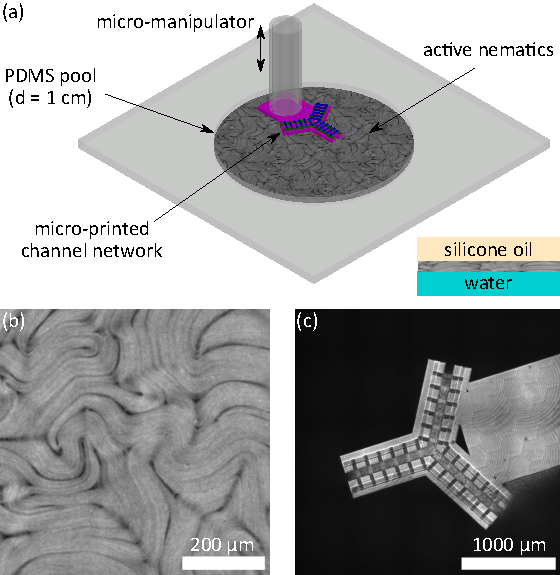
\includegraphics[width=0.45\textwidth]{2-bifurcation-experiment}
    \caption{
    \textbf{Confining microtubule-kinesin system at water-oil inerface -- the experimental setup.}
    (a) A schematic diagram of the experimental setup. 
    The microtubule-kinesin active nematic system is condensed at the water-oil interface, and is subject to lateral confinement by nano-printed channels. 
    (b) A schematic diagram of the bifurcation channels. 
    The Y-shape channel pattern is printed at the bottom.
    The ``bridges'' on the top are designed to hold the structure together. 
    (c) Top view of the bifurcation channels. 
    The relevant dimensions channel length $l=1000$ $\mu$m and channel width $w=100$ $\mu$m are labeled in place. 
    (d) A confocal image of a mature interfacial microtubule-kinesin system. 
    (e) A confocal image of the bifurcation channels set on the interfacial microtubule-kinesin system. 
    }
    \label{fig:bifurcation-experiment}
\end{figure}

We use the microtubule-kinesin mixture as the model active matter system. 
The microtubule-kinesin system is a well-established model system for active nematics \cite{Sanchez2012,Keber2014,Decamp2015,Hardouin2020}.
Active nematics are typically prepared at water-oil interface, as illustrated in Fig.~\ref{fig:bifurcation-experiment}(a). 
The ``grid'' of channels are printed using a high resolution 3D printer (Nanoscribe Photonic Professional GT2).
Figure~\ref{fig:bifurcation-experiment}(b) shows the design of a typical bifurcation channels.
The bottom layer of the printed structure is a Y-shape channel, while the top layer is a set of ``bridges'' that hold the structure together.
The middle layer is a set of spacers that separate the top and bottom layers, which keeps the bridges at a safe distance from the active nematics system.
Figure~\ref{fig:bifurcation-experiment}(c) shows a top view of the bifurcation channels.
All the three channels are of the same width $w=100\,\mu$m, while the length of the channels are $l=1000\,\mu$m.
An unperturbed active nematics system is shown in Fig.~\ref{fig:bifurcation-experiment}(d), while the same system with the bifurcation channels set in is shown in Fig.~\ref{fig:bifurcation-experiment}(e).

The active nematics system is observed using a confocal microscope (Nikon), and images are taken at 2 Hz using a 10X objective lens.
In a typical image, the field of view covers a part of all the bifurcation channels.
Then, \SI{400}{\micro\meter} of each channel is cropped and analyzed by PIV, as shown in Fig.~\ref{fig:bifurcation-symmetric}(a).

\section{Results}

\subsection{Symmetric bifurcation}

We first study the flow behavior at a symmetric bifurcation, where all the channels are of the same length.
The flow rates in the channels are plotted in Fig.\ref{fig:bifurcation-symmetric}(b).
The blue, orange and green curves represent the flow rates in channels A, B and C, respectively, corresponding to the colors of the borders in Fig.\ref{fig:bifurcation-symmetric}(a).
The light and thin curves in the back are the real flow rates, while the strong and thick curves in the front are Gaussian-smoothed flow rates with $\sigma=25$ s.
The gray curve is the sum of the flow rates in the 3 channels, which is used to verify the continuity at the junction.
Due to the variation of active nematics activity, the flow rates fluctuates in time. 
To normalize the flow rates of different magnitudes, we define a normalizer as the maximum of the smoothed absoluted flow rates in A, B and C, as indicated by the red curve. 
By dividing the flow rates by the normalizer, we obtain the normalized flow rates, which are used to construct the flow rate histogram.
In Fig.\ref{fig:bifurcation-symmetric}(c), we show the histogram of the normalized flow rates.
Instead of having a few sharp peaks, which was expected from the theoretical model \cite{Woodhouse2017}, the histogram shows a broad and even distribution of flow rates, covering most of the possible configurations of flow rates in the 3 channels for $\phi_A<0$.
Although the channels are designed to be fully symmetric, the grid requires a base structure to which the micromanipulator is attached, which may introduce some asymmetry in the flow rates.
Note that the flow rates in the 3 channels satisfy $\phi_A+\phi_B+\phi_C = 0$, so the histograms are not independent.
Therefore, in the following figures, we only show the $\phi_B$-$\phi_C$ histogram.

\begin{figure*}[!h]
    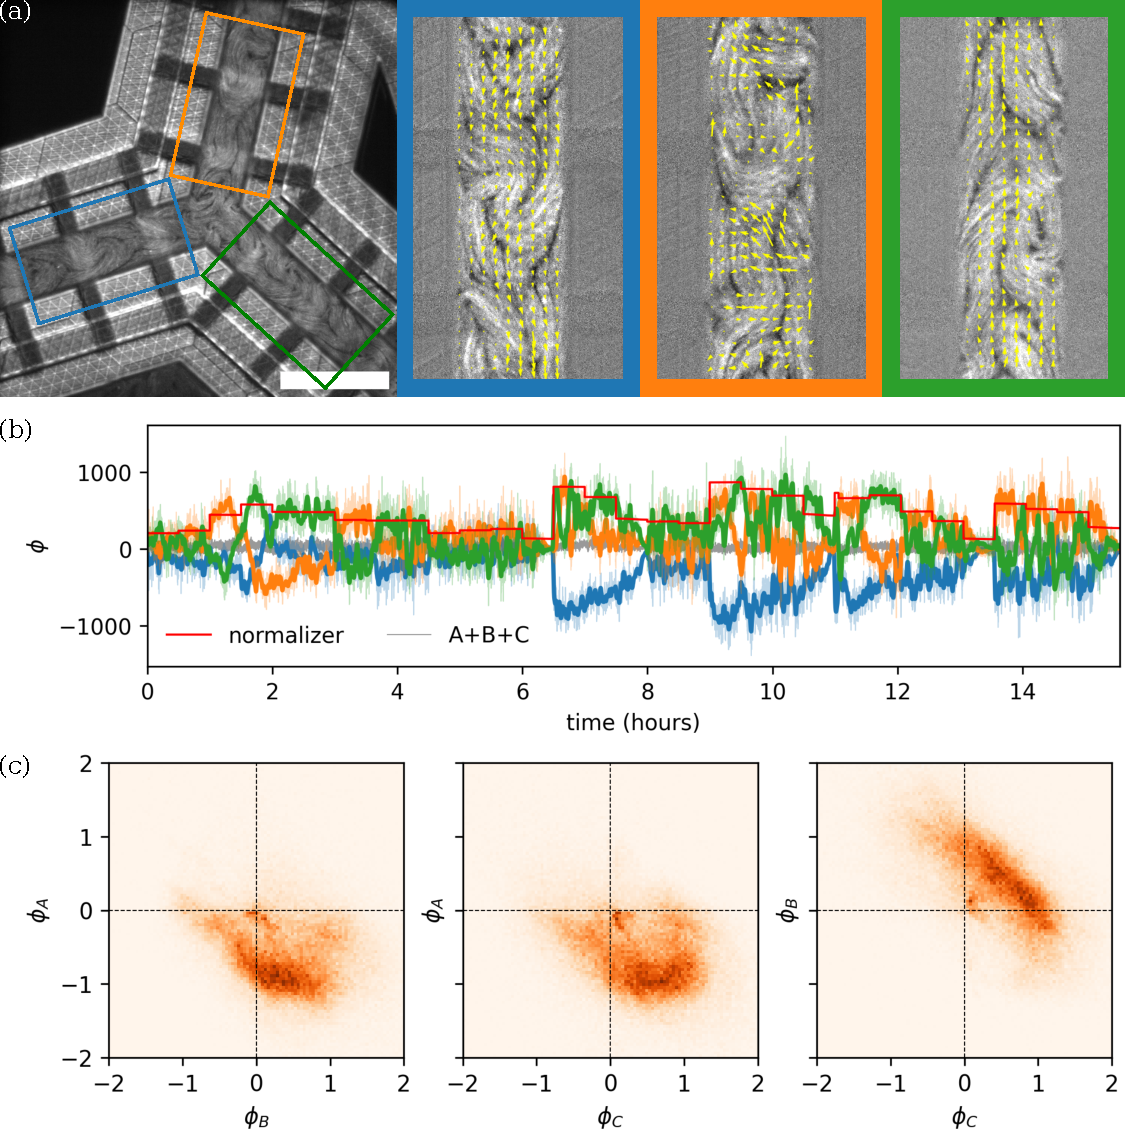
\includegraphics[width=\textwidth]{3-bifurcation-symmetric}
    \caption{
    \textbf{Flow rate measurements and flow rate histogram.}
    (a) A snapshot of microtubule-kinesin system confined in bifurcation channels.
    The scale bar is 200 $\mu$m.
    The 3 panels on the right are crops of each channel with corresponding border colors. 
    The yellow arrows are the results from PIV analysis. 
    (b) Flow rate time series in the 3 channels A (blue), B (orange) and C (green). 
    The light and thin curves in the back are the real flow rates, while the strong and thick curves in the front are Gaussian-smoothed flow rates with $\sigma=25$ s. 
    The red curve is the ``normalizer'', defined as the maximum of the   smoothed absoluted flow rates in A, B and C. 
    The gray curve is the sum of the flow rates in the 3 channels, which is used to verify the continuity at the junction.
    The unit of flow rate is $\mu$m$^2$/s.
    Note that the direction away from the junction is defined as the positive direction. 
    (c) The histogram of normalized flow rates. From left to right $\phi_A$-$\phi_B$, $\phi_A$-$\phi_C$ and $\phi_B$-$\phi_C$. Note that these histograms are not independent since the 3 flow rates satisfy $\phi_A+\phi_B+\phi_C = 0$. Therefore, in the following, we only show $\phi_B$-$\phi_C$ histogram.
    \textcolor{red}{Down size this figure and the figures in the following. No need to show flow rate time series. Labels can be relaxed.}
    }
    \label{fig:bifurcation-symmetric}
\end{figure*}

\subsection{Straight channel length}

Having learned from the fully symmetric bifurcation experiment, we enforce channel A as a ratchet channel, which guarantees that $\phi_A<0$.
We then study the effect of channel length on the flow behavior.
In Fig.\ref{fig:straight-channel-length}(a), we show the flow behavior at a 9-teeth ratchet inlet with 2 equal length outlets.
The flow fluctuates between polarized and non-polarized states, exploring all the possible configurations.
The equal splitting state is the most probable configuration.
It is also noticed that channels B and C are always outlets when fixing A as the inlet with ratchets.
This observation implies that the ratchet channel has a dominant effect on the flow behavior, compared to the straight channels.
Such dominance will be further confirmed in the following experiments.
In Fig.\ref{fig:straight-channel-length}(b), we show the flow behavior at a 4-teeth ratchet inlet with long and short outlets.
The expectation from theory is that the flow will prefer the longer outlet, as the longer path has a lower energy state and is therefore more energetically favorable.
However, we observe that the flow explores all the possible configurations, showing no preferred splitting ratio.
In Fig.\ref{fig:straight-channel-length}(c), we show the flow behavior at a 4-teeth ratchet inlet with 2 equal length outlets.
This experiment is done to keep consistent ratchet numbers in the inlet to avoid the potential effect of ratchet number on the flow behavior.
The resulting flow configuration is very similar to the longer ratchet inlet one though: the flow fluctuates between polarized and non-polarized states, exploring all the possible configurations.

\begin{figure*}[!h]
    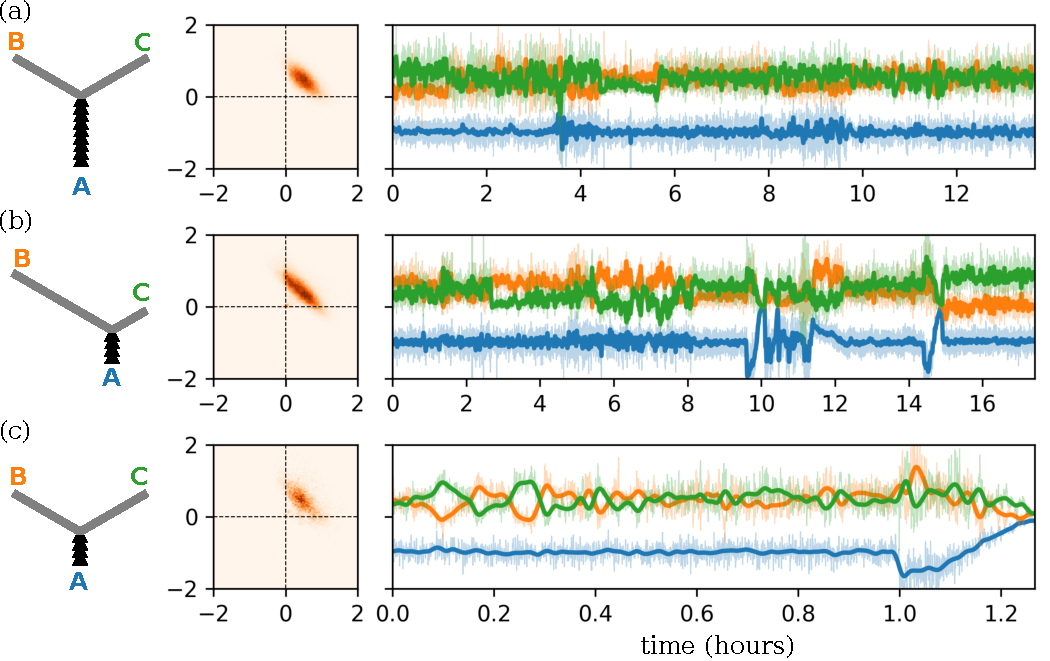
\includegraphics[width=\textwidth]{4-straight-channel-length}
    \caption{
    \textbf{Ratchet inlet and straight outlets: histogram and time series.}
    (a) 9-teeth ratchet inlet with 2 equal length outlets. 
    The flow fluctuates between polarized and non-polarized states, exploring all the possible configurations.
    The equal splitting state is the most probable configuration.
    (b) 4-teeth ratchet inlet with long and short outlets.
    The flow also explores all the possible configurations, but shows no preferred splitting ratio.
    (c) 4-teeth ratchet inlet with 2 equal length outlets.
    The flow fluctuates between polarized and non-polarized states, exploring all the possible configurations.
    The equal splitting state is the most probable configuration.
    }
    \label{fig:straight-channel-length}
\end{figure*}

\subsection{Ratchet inlet and outlets}

We then study the flow configurations of active nematics in bifurcation channels with ratchet inlets and outlets.
The experimental results are shown in Fig.\ref{fig:ratchet-dominance}.
A general observation is that the peaks in the histograms are sharp, indicating that the flow configurations are more deterministic than in straight channels.
When the outlet channels have different numbers of ratchet, as shown in Fig.~\ref{fig:ratchet-dominance}(a) the flow robustly splits into different fractions in the two outlet channels.
Interestingly, the flow rate ratio in the two outlet channels is almost equal to the ratio between the number of ratchet teeth.
Does this unequal splitting of flow arise from the difference in the length of the channels?
To answer this question, we keep the channels lengths unchanged, but modify the number of ratchet teeth in channel B, so that channels B and C has the same number of ratchet teeth.
In this case, the flow robustly split into the two outlet channels with a 1:1 ratio, as shown in Fig.\ref{fig:ratchet-dominance}(b).
This result suggests that the ratchet teeth in the outlet channels play a dominant role in determining the flow behavior at bifurcations.
In Fig.\ref{fig:ratchet-dominance}(c), we show the flow behavior in channels with equal length and number of ratchet teeth.
The flow again splits with a 1:1 ratio, confirming the dominant role of ratchet teeth.

\begin{figure*}[!h]
    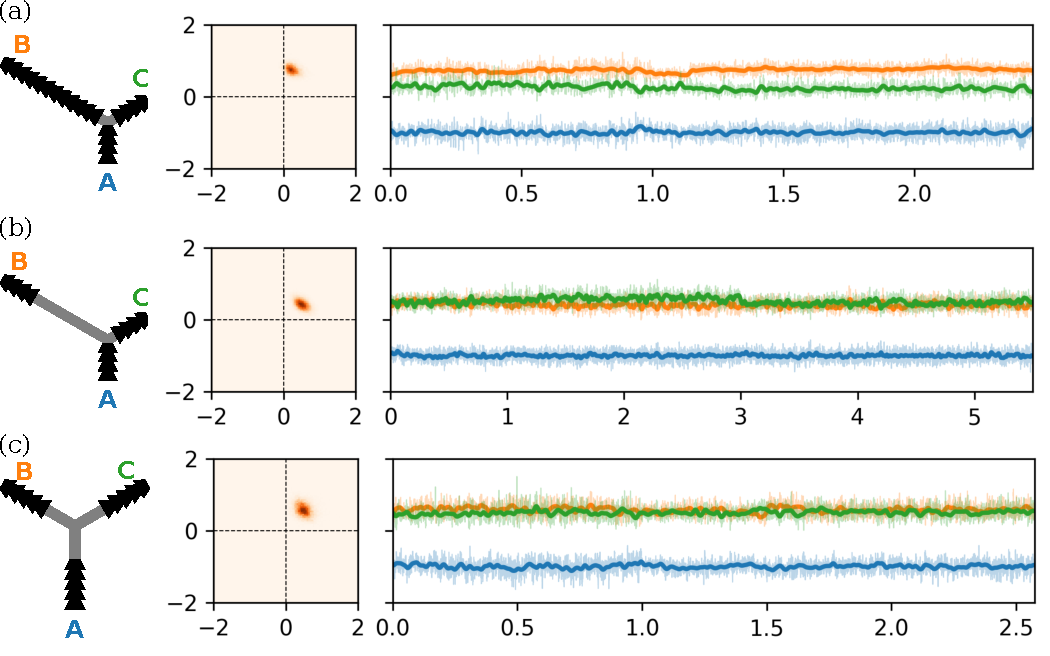
\includegraphics[width=\textwidth]{5-ratchet-dominance}
    \caption{
    \textbf{Ratchet inlet and outlets: histogram and time series.}
    (a) The numbers of ratchet teeth in channels A, B and C are 4, 13 and 4, respectively. 
    Let's refer to this bifurcation channel network 4-13-4 bifurcation. 
    In contrast to straight channels, the flows exhibit a sharp peak in the histogram, while other splitting ratios remain rarely explored. 
    The splitting ratio is around 3:1.
    (b) 4-4-4 bifurcation, where channel B has an extended straight portion. 
    The flows again exhibit a sharp peak in the histogram at a splitting ratio around 1:1.
    (c) 5-5-5 bifurcation, where all the channels are of the same length. 
    The flows again exhibit a sharp peak in the histogram at a splitting ratio around 1:1.
    }
    \label{fig:ratchet-dominance}
\end{figure*}

\begin{figure*}[!ht]
    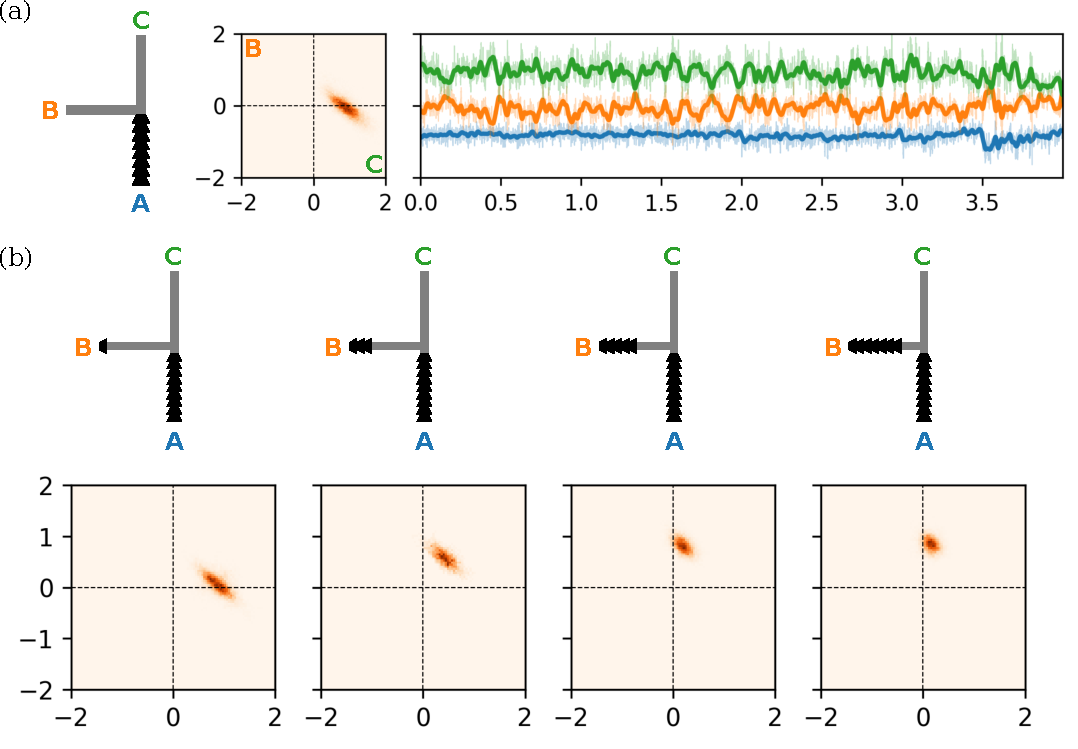
\includegraphics[width=\textwidth]{6-angle-ratchet-competition}
    \caption{
    \textbf{The role of turning angles.}
    (a) A bifurcation with a 9-teeth ratchet inlet and 2 straight outlets of the same length. 
    The outlets have different turning angles with respect to the inlet channel A: $\angle AOB=90^\circ$ and $\angle AOC=180^\circ$.
    The flow rate histogram and time series suggest that the flow prefers the $180^\circ$ channel C, i.e. the channel parallel to the inlet channel A, rather than channel B which requires a $90^\circ$ turn. 
    (b) Adding various numbers of ratchets to channel B to compete with the $90^\circ$ turning angle. 
    From left to right, 1, 3, 5, 7 ratchet teeth are added to the end of channel B. 
    Below the schematics of bifurcation channels are the $\phi_B$-$\phi_C$ flow rate histograms corresponding to the design above. 
    As the number of ratchet teeth in channel B is increased, the splitting ratio between B and C is increase from 0 to $\infty$.
    }
    \label{fig:angle-ratchet-competition}
\end{figure*}

\bibliography{ref}
\bibliographystyle{unsrtnat}

\end{document}
%
% ****** End of file apssamp.tex ******